\clearpage
\subsubsection{MSVC + \olly}
\index{\olly}

\RU{Я обвел красным в стеке 2 пары 32-битных слов, каждая пара --- 
это double-числа в формате IEEE 754 переданные из \main.}
\EN{I marked by red 2 pairs of 32-bit words in stack. Each pair is double-number in
IEEE 754 format passed from \main.}
\RU{Видно, как первая \FLD загружает значение ($1.2$) из стека и помещает в регистр \ST{0}:}
\EN{We see how first \FLD loads a value ($1.2$) from stack and put it into \ST{0} register:}

\begin{figure}[H]
\centering
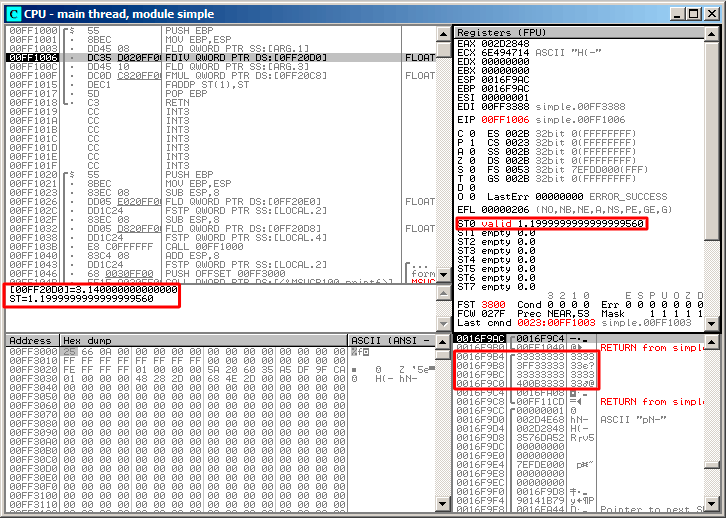
\includegraphics[scale=\FigScale]{patterns/12_FPU/1_simple/olly1.png}
\caption{\olly: \RU{первая \FLD исполнилась}\EN{first \FLD executed}}
\label{fig:FPU_simple_olly_1}
\end{figure}

\RU{Из-за неизбежных ошибок конвертирования числа из 64-битного IEEE 754 в 80-битное (внутреннее в FPU),
мы видим здесь $1.1999...$, что очень близко к $1.2$.}
\EN{Because of unavoidable conversion errors from 64-bit IEEE 754 float point number into 80-bit
(used internally in FPU), we see here $1.999...$, which is close to $1.2$.}
\RU{Прямо сейчас \EIP указывает на следующую инструкцию (\FDIV), загружающую double-число (константу) 
из памяти.}
\EN{\EIP right now is pointing to the next instruction (\FDIV), which loads double-number (a constant)
from memory.}
\RU{Для удобства}\EN{For convenience}, \olly \RU{показывает её значение}\EN{shows its value}: $3.14$.

\clearpage
\RU{Трассируем дальше}\EN{Let's trace more}. 
\FDIV \RU{исполнилась}\EN{executed}, \RU{теперь}\EN{now} \ST{0} \RU{содержит}\EN{contain} $0.382...$ 
(\gls{quotient}):

\begin{figure}[H]
\centering
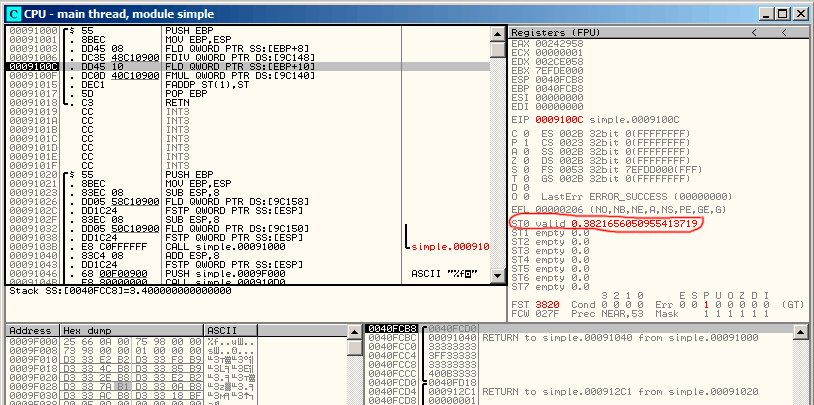
\includegraphics[scale=\FigScale]{patterns/12_FPU/1_simple/olly2.png}
\caption{\olly: \FDIV \RU{исполнилась}\EN{executed}}
\label{fig:FPU_simple_olly_2}
\end{figure}

\clearpage
\RU{Третий шаг}\EN{Third step}: \RU{вторая}\EN{the next} \FLD 
\RU{исполнилась, загружая в \ST{0} $3.4$ (мы видим приближенное число $3.39999...$)}
\EN{executed, loading $3.4$ into \ST{0} (we see here approximated value $3.39999...$)}: 

\begin{figure}[H]
\centering
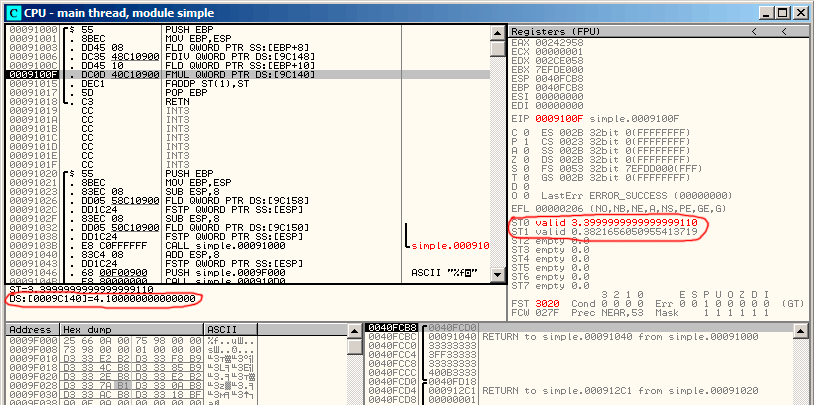
\includegraphics[scale=\FigScale]{patterns/12_FPU/1_simple/olly3.png}
\caption{\olly: \RU{вторая \FLD исполнилась}\EN{second \FLD executed}}
\label{fig:FPU_simple_olly_3}
\end{figure}

\RU{В это время}\EN{At the same time,} \gls{quotient} \IT{\RU{провалилось}\EN{pushed}} 
\RU{в}\EN{into} \ST{1}.
\RU{\EIP в это время указывает не следующую инструкцию}\EN{Right now, \EIP points to the next
instruction}: \FMUL. 
\RU{Она загружает константу}\EN{It loads} $4.1$ \RU{из памяти, так что \olly тоже показывает её здесь}
\EN{constant from memory, so \olly shows it here}.

\clearpage
\RU{Затем}\EN{Next}: \FMUL \RU{исполнилась, теперь в \ST{0} произведение}
\EN{was executed, now \gls{product} is in \ST{0}}:

\begin{figure}[H]
\centering
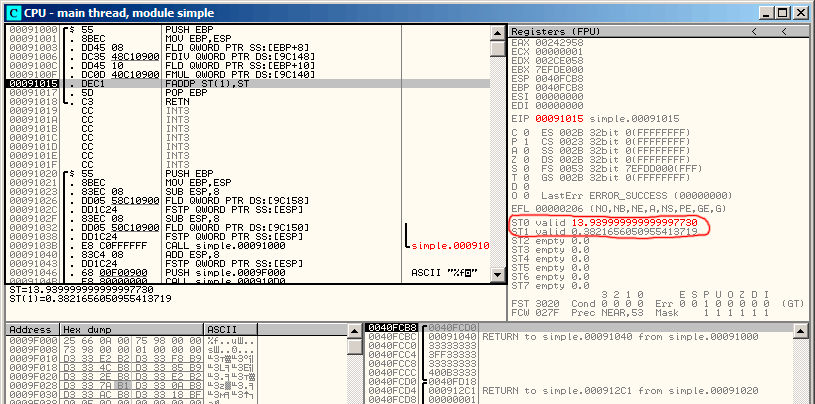
\includegraphics[scale=\FigScale]{patterns/12_FPU/1_simple/olly4.png}
\caption{\olly: \FMUL \RU{исполнилась}\EN{executed}}
\label{fig:FPU_simple_olly_4}
\end{figure}

\clearpage
\RU{Затем}\EN{Next}: \FADDP \RU{исполнилась, теперь в \ST{0} сумма, а \ST{1} очистился}
\EN{was executed, now result of addition is in \ST{0}, and \ST{1} is cleared}:

\begin{figure}[H]
\centering
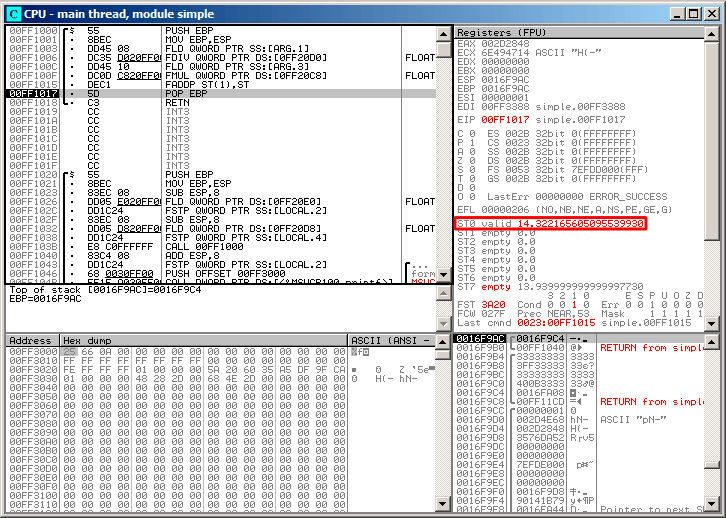
\includegraphics[scale=\FigScale]{patterns/12_FPU/1_simple/olly5.png}
\caption{\olly: \FADDP \RU{исполнилась}\EN{executed}}
\label{fig:FPU_simple_olly_5}
\end{figure}

\RU{Сумма остается в \ST{0}, потому что ф-ция возвращает результат своей работы через \ST{0}.}
\EN{Result is left in \ST{0}, because the function returns its value in \ST{0}.}
\RU{Позже, \main возьмет это значение оттуда.}
\EN{\main will take this value from the register soon.}\\
\\
\RU{Мы также видим кое-что необычное: значение $13.93...$ теперь находится в \ST{7}.}
\EN{We also see something unusual: $13.93...$ value is now located in \ST{7}.}
\RU{Почему}\EN{Why}?

\label{FPU_is_rather_circular_buffer}
\RU{Я писал, что регистры в \ac{FPU} представляю собой стек}\EN{As I wrote before, \ac{FPU} registers
is stack}: \ref{FPU_is_stack}. 
\RU{Но это упрощение}\EN{But this is simplification}.
\RU{Представьте, если бы \IT{в железе} было бы так, как описано, тогда при каждом заталкивании 
(или выталкивания) в стек,
все остальные 7 значений нужно было бы передвигать (или копировать) в соседние регистры, 
а это слишком много работы.}
\EN{Just imagine if it would be implemented \IT{in hardware} as it's described, 
then all the rest 7 register's
contents must be moved (or copied) to adjacent registers during pushing and popping, 
and that's a lot of work.}
\RU{Так что в реальности,
\ac{FPU} имеет просто 8 регистров и указатель (называемый \TT{TOP}), содержащий номер регистра,
которая в текущим момент является ``вершиной стека''.}
\EN{In reality, \ac{FPU} has just 8 registers and a pointer (called \TT{TOP}) which has register number,
which is current ``top of stack''.}
\RU{При заталкивании значения в стек, регистр \TT{TOP} меняется, и указывает на свободный регистр, 
затем значение записывается в этот регистр.}
\EN{When value is pushed into stack, \TT{TOP} register is changing and pointing to a next available register,
and then a value is written to it.}
\RU{При выталкивании значения из стека, процедура обратная, однако, освобожденный регистр не обнуляется}
\EN{The procedure is reversed if value is popped, however, register which was freed is not cleared}
(\RU{наверное, можно было бы сделать, чтобы обнулялся, но это лишняя работа и работало бы медленнее}\EN{it 
could be cleared, but this is another work which may degrade performance}).
\RU{Так что это мы здесь и видим}\EN{So that's what we see here}. 
\RU{Можно сказать, что \FADDP сохранила сумму, а затем вытолкнуло один элемент.}
\EN{It can be said, \FADDP saved sum in stack, and then popped one element.}
\RU{Но в реальности, эта инструкция сохранила сумму и затем передвинула регистр \TT{TOP}.}
\EN{But in fact, this instruction saved sum and then shifted \TT{TOP} register.}
\RU{Было бы еще точнее сказать, что регистры \ac{FPU} представляют собой кольцевой буфер.}
\EN{More precisely, \ac{FPU} registers is circular buffer.}
